\chapter{Introducción a las relaciones}
Podemos diseñar relaciones entre los objetos de las diferentes clases de objetos.
Estas relaciones pueden ser muy diferentes entre sí, habiendo algunas más estrictas
que otras.
\vspace*{0.2cm}
\begin{figure}[h]
  \begin{minipage}{0.4\textwidth}
    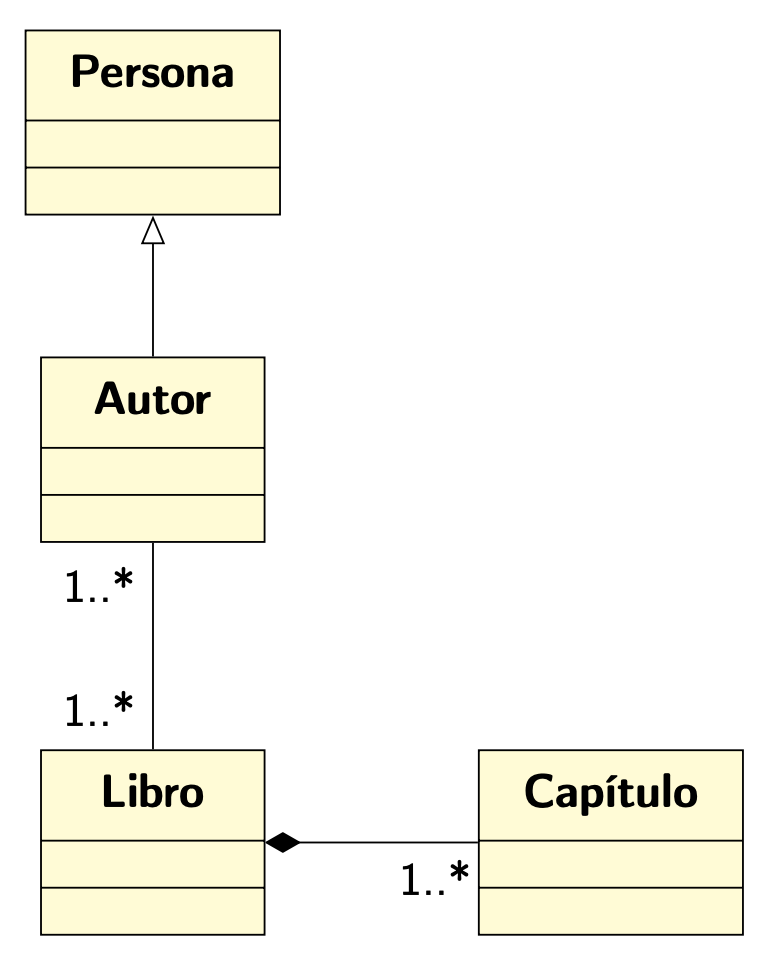
\includegraphics[width=\textwidth]{Imagenes/intro1.png}
    \caption{Diagrama de Clases}
  \end{minipage}
  \begin{minipage}{0.6\textwidth}
      \vspace{-6\baselineskip} % ajusta la posición vertical del texto
    Al conjunto de relaciones entre las diferentes clases de datos, lo denominamos →\textit{diagramas de clases}.\\
    
	Aquí encontramos varios tipos de relaciones (asociaciones, generalizaciones, composiciones, etc.).\\
	
	Entre las diferentes clases encontramos enlaces de objetos, los cuales contienen una multiplicidad y dirección.\\
	
	Los objetos se \textbf{enlazan} y las clases se \textbf{relacionan}.
  \end{minipage}
  
\end{figure}
Por defecto la relación es \textbf{bidireccional} por tanto, tenemos que incluir la relación en ambas clases, si no fuera así (es decir unidireccional) solamente se define la relación y los métodos necesarios en la clase opuesta a la "flecha".